\documentclass[12pt]{article}
\usepackage{verbatim}
\usepackage[dvips]{epsfig}
\usepackage{color}
\usepackage{url}
\usepackage[colorlinks=true]{hyperref}

\begin{document}

\section*{GENESIS: Documentation}

{\bf Related Documentation:}
% start: userdocs-tag-replace-items related-do-nothing
% end: userdocs-tag-replace-items related-do-nothing

\subsection*{Figure\,9}

\begin{figure}[h]
\centering
   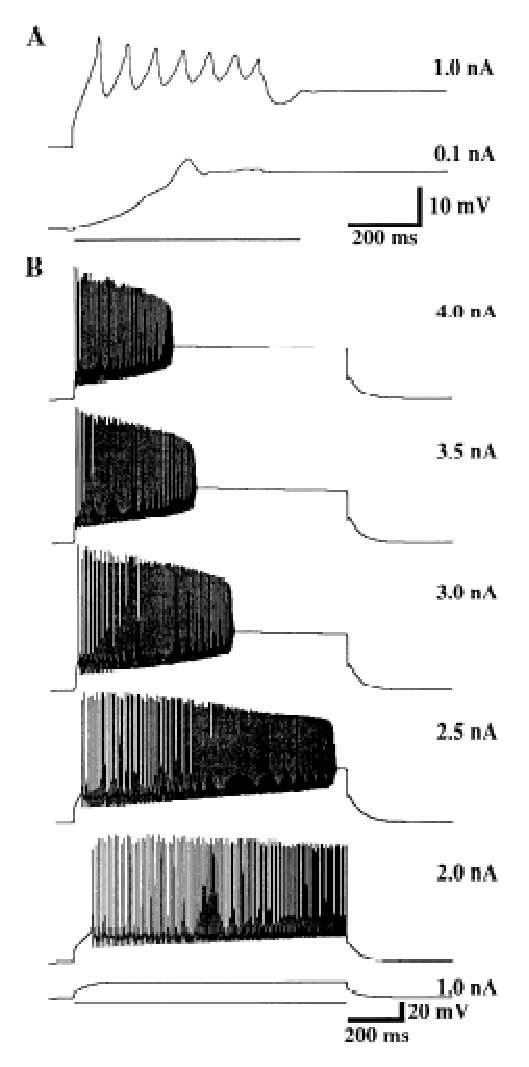
\includegraphics[scale=0.65]{figures/Fig.1.9.eps}
   \caption{Simulation of channel blocking experiments. {\it A}: Simulation of the effect of blocking Na$^+$ currents by tetrodotoxin (TTX) application. {\it B}: Simulation of the effect of blocking Ca$^{2+}$ currents by Co$^{2+}$ or Cd$^{2+}$ application. Membrane potential in the soma during current injections of indicated amplitudes in the soma.}
   \label{fig:DS1.9}
\end{figure}

\bibliographystyle{plain}
\bibliography{../tex/bib/g3-refs.bib}

\end{document}
